\chapter{Introduction}
\pagenumbering{arabic}
\setcounter{page}{1}
% general introduction to the problem
Human pose estimation aims at detecting the pose or skeleton of a person based on visual information only. It finds many applications, from games to medical applications\cite{kumarapu2020animepose, ClinicalApplicationChen, MedicalAnimation}. However, human pose estimation is a difficult task that is prone to errors\cite{HPEIsHard}. These errors can be caused by different factors, such as the environment, the camera, and the person. These errors can cause the joints of the pose to be in the incorrect position or missing. This can cause the pose estimation to be incorrect, and therefore, the human-computer interaction will be hampered. The goal of this thesis is to develop a method that allows for the detection of these errors such that the pose information can either be improve on them or that or be handled accordingly.

One of the limiting factors for human pose estimation is the user itself. If the posture is not as the model expects then errors might occur. This is especially true for applications that are designed for rehabilitation and exercise purposes. In these applications, the user is often elderly and has limited mobility, as is the case for games developed by SilverFit\footnote{\url{https://www.silverfit.com/en/}}. SilverFit is a serious gaming company that develops games for rehabilitation with a special focus on geriatric patients. In their games, SilverFit uses human pose estimation to detect the pose of the player and use it to control the game to make exercise more enjoyable while promoting activity. This thesis is written in colaboration with SilverFit and aims at improving the human pose estimation by giving featback on the errors in their games.

For some exercises designed by SilverFit and other companies, human pose estimation is not sufficiently reliable to create an enjoyable experience for patients in every environment. Especially sedentary exercises often cause the human pose estimation to fail or to produce unreliable results.

In this chapter, the research question that is answered in this thesis is discussed. Furthermore, the procedure with which the research question is answered is laid out. Finally, the fundamentals of human pose estimation and the metrics that are used to analyse the results are discussed, and related work is presented.


\subsubsection{Applications of human pose estimation}
% Should be in the introduction and not headers necessary
Human pose estimation finds application in many different fields. In this chapter some of the most common applications of human pose estimation are mentioned.

\paragraph{Gaming and entertainment}

Gaming and entertainment is one of the most common applications of human pose estimation. Games can use human pose estimation in a way that makes the interaction between humans and computers very natural. One of the systems that kickstarted the use of depth cameras in games was the Xbox Kinect by Microsoft. The Kinekt used a depth camera to track the movement of the player and used this information to control the games. \cite[Citation needed]{}

However, since human pose estimation requires space and a good camera, it is not as wide spread as conventional input peripherals.

\paragraph{Autonomous Driving}

Autonomous driving has been in development ever since humans replaced horses with cars\cite{OldAutoDrive}. However, the development of autonomous driving has been very slow. The main reason for this is that autonomous driving requires a lot of information about the environment. This information is usually provided by sensors that are installed in the car. However, sensors alone do not always suffice. In some cases, cars need to be able to estimate the pose of a human to make a decision. The posture of a human can be used to determine the action and therefore the future trajectory of the person. 

\paragraph{Animation}

To exactly emulate human movements in animation, animators can either manually move the joints of a digital skeleton or they can use real human\footnote{Or animal} actors to provide the movement for them. The manual creation of realistic movement is oftentimes very time-consuming and also error-prone. Therefore, animators often use real human actors to provide the movement for them. This provides animators with a skeleton and movement which is accurate and does not include human error. In large production studios, this is often done with motion capture or MoCap. 

MoCap is a technique that uses cameras to capture the movement of a human actor. The cameras are placed around the actor and record the movement of the actor. The actor usually wears a suit that is covered with markers. These markers are used to determine the position of the actor. To reduce the amount of occlusion of the markers a large number of cameras are used. This allows the cameras to capture the movement of the actor from different angles. However, this also increases the price of development. In cases where MoCap is not a viable option, animators can use human pose estimation to estimate the pose of a human actor using cheaper RGB cameras or RGBD cameras.

\paragraph{Security}

Another application of human pose estimation is the detection of annomalous behaviour. The detection of such behaviour can be used to prevent security incidents in public spaces.

\paragraph{Healthcare}

To aid in the rehabilitation of patients as well as to improve the quality of life of elderly people, human pose estimation can be used to detect the pose of a person and provide feedback on the pose of the person during exercises.\cite{ClinicalApplicationChen}


\section{Research question}

As mentioned earlier, a major problem with human pose estimation is that it is not possible to tell if the joints are faulty or not. This is a problem for SilverFit, as they want to be able to tell if the joints are faulty or not. Using faulty joints can decrease the efficacy of the training effect of the developed games and can make them very frustrating to use and develop. A joint is considered faulty if it is not in the incorrect position, i.e. the distance from the theoretical position is greater than a chosen threshold, or if it missing from the skeleton.

In this thesis, we first ask what problems occur during human pose estimation and what common error sources are. We aim to find which problems are the most common and which joints are most affected by the errors. This will help give an overview of the issues related to human pose estimation and help develop ways to detect these issues. 

Once we know the issues that occur during human pose estimation, we aim to develop a method that can capture the camera stream in a way that allows us to label the data according to the exercise and environment it was captured in. This will allow us to create a dataset that can be used for future purposes.

Furthermore, we try to find if it is possible, given a joint, the RGB data, and the depth data, to determine if the joint is faulty or not.




\section{Process Pipeline}
\label{sec:process_pipeline}

The whole process of fault estimation can be seen as a pipeline. We start at the most basic starting block, the camera streams, and end at the most complex block, the fault estimation. The pipeline is shown in Figure \ref{fig:process_pipeline}. The pipeline consists of eight steps, which are described in more detail in the following sections. The steps are (\textbf{0}) Preliminary Analysis, (\textbf{I}) Stream Pre-Processing, (\textbf{II}) Data Acquisition, (\textbf{III}) Data Population, (\textbf{IV}) Data Post-Processing/Evaluation, (\textbf{V}) Data Augmentation, (\textbf{VI}) Model Training, and (\textbf{VII}) Model Evaluation. The results of each step are used as input for the next step. 

We further divided the process into a preliminary, data processing, and model development phase. The preliminary phase focuses on issue analysis and exercise development, the data processing phase is the first five steps of the pipeline. The model development phase is the last two steps of the pipeline.

In the next chapters, we give a basic overview of the whole process. We go into more detail in the following sections.

\begin{figure}[ht]
    \centering
    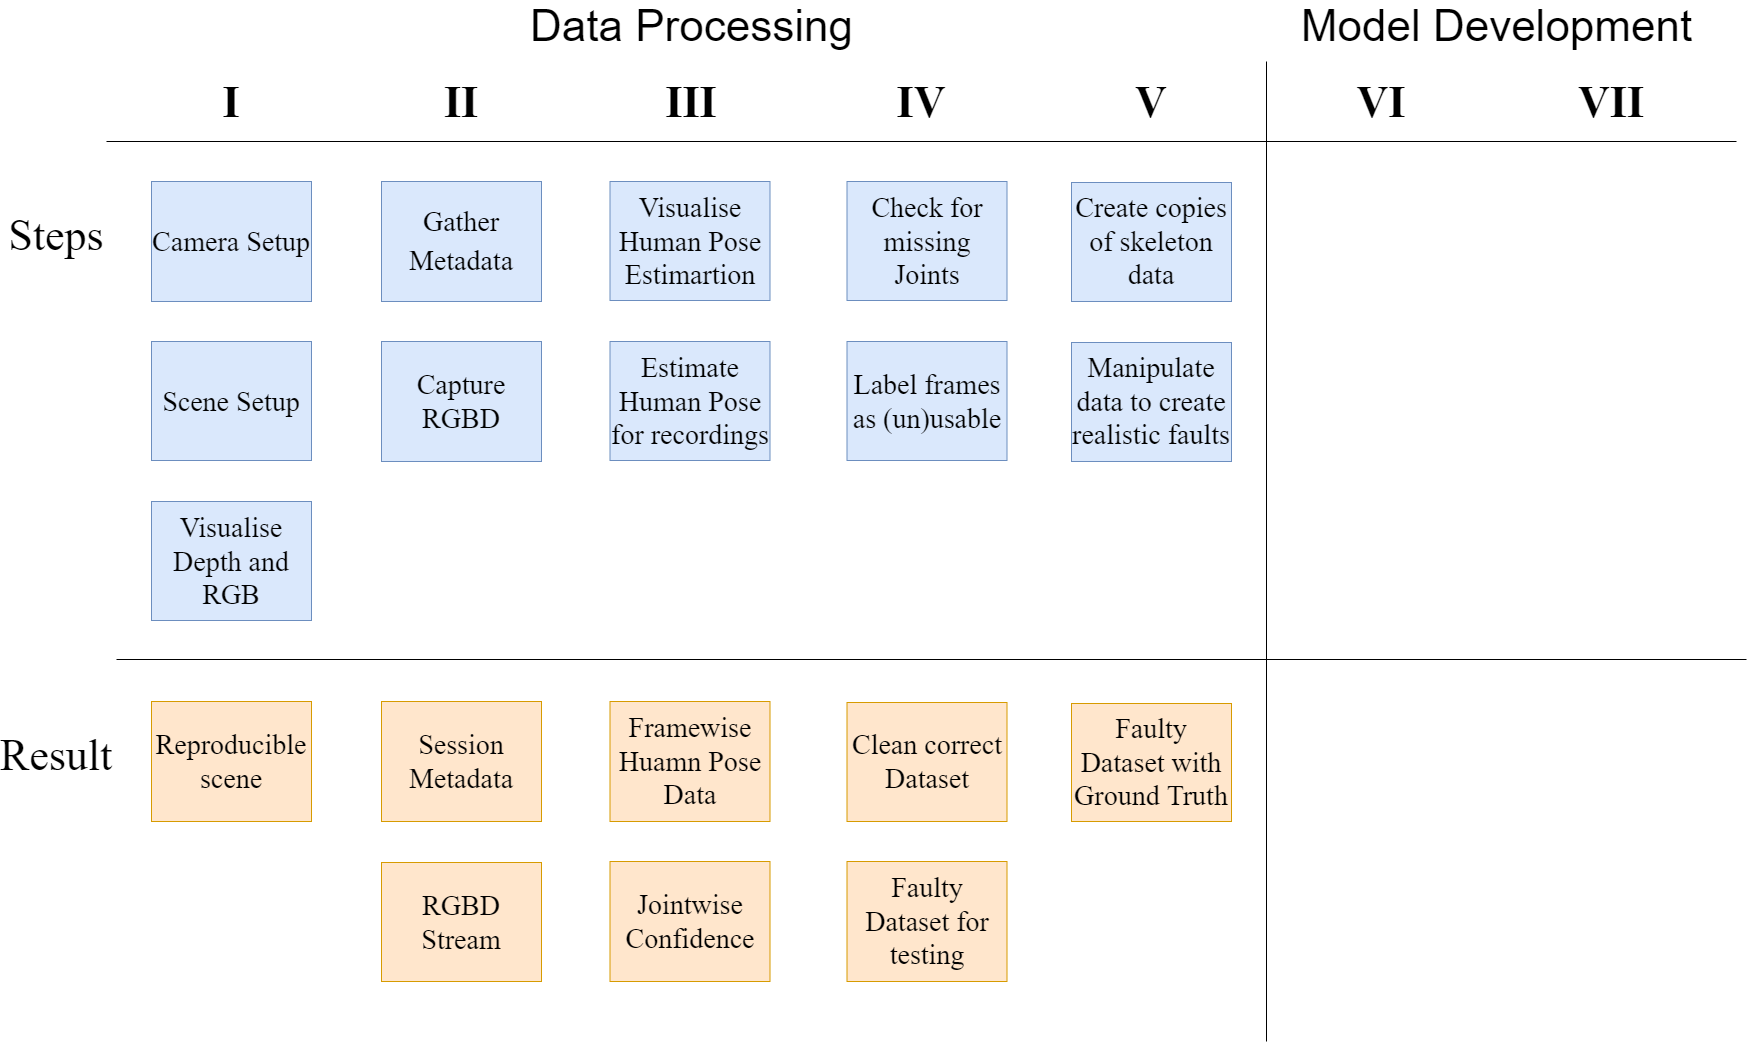
\includegraphics[width=\textwidth]{figures/ProcessingPipeline/ProcessingPipeline.png}
    \caption[Process Pipeline with all steps]{The whole Process pipeline with all the steps, which are marked in blue, and the results of each step, which are marked orange. The results of the steps are used as input for the next step. The steps are described in more detail in the following sections. The steps are: (\textbf{0}) Preliminary Analysis, (\textbf{I}) Stream Pre-Processing, (\textbf{II}) Data Acquisition, (\textbf{III}) Data Population, (\textbf{IV}) Data Post-Processing/Evaluation, (\textbf{V}) Data Augmentation, (\textbf{VI}) Model Training, and (\textbf{VII}) Model Evaluation.}
    \label{fig:process_pipeline}
\end{figure}

\section{Related Work}
\label{sec:related_work}

A plethora of methods have been developed to estimate the pose of a human. In this section, we will discuss some of the methods that have been developed to estimate the pose of a human. Additionally, we discuss datasets that have been developed to test the performance of the methods. Finally, we discuss some of the methods that have been developed to estimate the fault.

\subsection{Human Pose Estimation}


Human Pose Estimation using Iterative Error feedback. \cite{IterativeErrorFeedback}

While OpenPose developed Hand Pose\cite{OpenPoseHand} and also Multi-Person Human Pose Estimation \cite{OpenPoseMulti}, our main focus lies on their most recent pose estimator \cite{OpenPosePose} and their CNN network \cite{OpenPoseCNN}. Openpose uses affinity fields. The affinity fields are a set of 2D Gaussian distributions that are used to estimate the pose of a human. The affinity fields are used to estimate the pose of a human by estimating the probability of a joint being in a certain location. The probability of a joint being in a certain location is calculated by summing the probability of the joint being in that location for each of the Gaussian distributions.

\subsubsection{Reviews}


A review of point cloud-based human pose estimation \cite{ReviewPointcloudHPE}

A review of 2D human pose estimation methods \cite{ReviewHPE}

\subsubsection{RGB Pose Estimation}

\cite{RGBHPE}

But we wont go into much detail as we focus on RGBD data.

\textbf{This is a bit wrong, the dataset is multi modal but the definition of multimodal is different in this method, it means RGB plus D and not different angles sometimes maybe not, read it through again:}
The limited number of multi-modal datasets causes the existence of human pose estimators for cameras from different angles to be small. One example of multi-modal human pose estimation was introduced by Jingxiao Zheng et al.\cite{MultiModalHPERGBD}. In their paper 

\subsubsection{RGBD Pose Estimation}

\textbf{This is a bit out of context:}
As mentioned by Jingxiao Zheng et al. in \cite{MultiModalHPERGBD}, the key points or joints of the skeleton do not lay on the surface of the person and therefore the determination of the exact position of the joints are not a direct projection on the depth image or the point cloud.

\cite{PASCUALHERNANDEZ2022102225}

\cite{RGBDHPEforRoboticTaskLearning}

Nuitrack does not offer any white paper or documentation on their method. However, they have written that they use a CNN to estimate the pose of a human. That CNN uses both RGB and depth information to estimate the pose of a human.


\subsection{RGBD CNNs}

Early HPE algorithm uses trees \cite{EarlyRGBDHPE}

CNNs more useful for images and stuff. Cnns are not a new invention yada yada yada \cite{OldCNN}. But like many things in the neural network Biz, they were limited by the hardware available at the time. They have since formed the basis of many new methods in computer vision, such as Human Pose estimation. Especially AlexNet \cite{AlexNet} and VGG \cite{VGG} proved the potential of CNNs in Computer Vision tasks. 

\subsection{Object Detection}

\cite{3DCNNSalient} Proposes different methods of fusion for RGBD data.

\subsubsection{Depth Completion}

Realsense with Tensorflow \cite{TensorflowRealsense} uses U-Net for depth completion \cite{UNET}.

\subsubsection{Action Recognition}

Cool CNN --> \cite{ElboushakiAbdessamad2020MAmf}

Another Review on human pose estimation but this time it is for action recognition \cite{ReviewHPEforActionRecognition}

Great input fusion graphic \cite{ActionRecognitionHPEFusion}

\subsection{Fault Estimation}

Human3.6M: Large Scale Datasets and Predictive Methods for 3D Human Sensing in Natural Environments \cite{h36m_pami}


Latent Structured Models for Human Pose Estimation \cite{IonescuSminchisescu11} 

\section{Fundamentals}
\label{sec:fundamentals}

In this section, the fundamentals that are necessary to understand the thesis are discussed. These fundamentals are human pose estimation, the fundamentals of machine learning, and the evaluation metrics that are used to evaluate the results. 

\subsection{Human pose estimation}

There is a wide variety of how humans can interact with computers. Ranging from early punch cards to touch screens, the methods have evolved to be more natural and intuitive. In recent years, the use of cameras has become more popular, since they require no physical contact with a computer and therefore allow users to seamlessly interact with an application.

\subsubsection{Pose visualisation}

Different methods to capture the pose of a human have been developed. Depending on the usage of the pose estimation, different methods are used to visualise the pose of a human. These visualisations may provide different information about the pose of a human.

There are mainly three different ways the human pose can be visualised. The first and most basic way is to visualise the pose as a kinematic representation, in which a "skeleton" with bones and joints is used to represent the pose of a human. The skeleton is made up of joints, which are connected by bones. The number of joints and bones can vary, but the most common skeleton is made up of 17 joints and 16 bones, as can be seen in figure \ref{fig:pose_example}. The joints are usually labelled with a number, which is used to identify the joint in the output of the pose estimation. The representation of a joint in the data varies, but it is usually a 2D or 3D point in space. In some cases, an additional joint representation is provided with a keypoint orientation that enables the clear representation of all degrees of freedoms joints have\cite{KeypointOrientation}. Additionally, in some cases, especially if the human pose was estimated using a neural network, a confidence rating or score is added which can be used to determine the reliability of the joint.

\begin{figure}
    \centering
    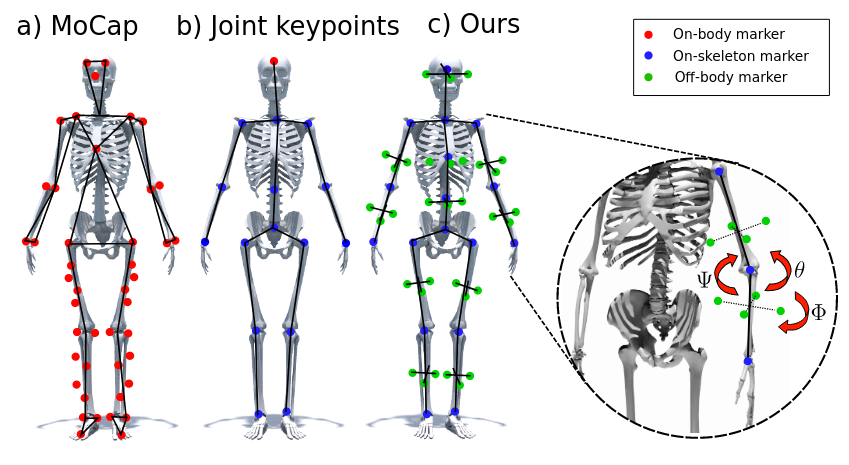
\includegraphics[width=0.8\linewidth]{figures/HPE/PoseExample.png}
    \caption[Example for human Pose estimation]{Example of a human pose captured with different methods. (a) A captured skeleton using MoCap (b) A traditional human skeleton representation. (c) A pose representation that includes the orientation of the joints as well as the bones as presented by Martin Fish and Ronald Clark\cite{KeypointOrientation}}
    \label{fig:pose_example}
\end{figure}

The second way to visualise a human pose is by using a 2D silhouette or 2D rectangles and shapes. These methods are also called contour-based methods. An example of contour-based methods was introduced by Yunheng Liu\cite{contourHPE}. Contour-based methods are often used in combination with a skeleton representation. The skeleton is used to determine the location of the joints, while the contour is used to determine the shape of the body. This is useful when the skeleton is not able to determine the shape of the body, for example, when the person is wearing a coat or a jacket. This is also used for some games developed by SilverFit.

Finally, the third way to represent a human pose is with a three-dimensional volume. This volume may be simple cylindrical shapes or a body mesh. A body mesh is a 3D representation of the body, which is made up of vertices and triangles. The three different representations of the human pose can be seen in figure \ref{fig:pose_representation}.

\begin{figure}
    \centering
    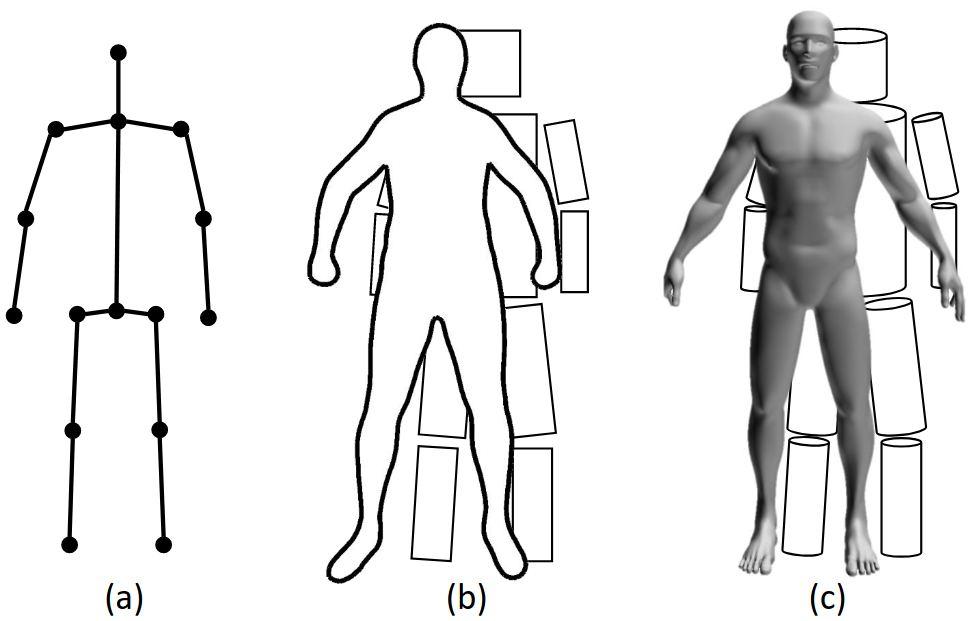
\includegraphics[width=0.8\linewidth]{figures/HPE/PoseRepresentation.png}
    \caption[Different representations of the human pose]{Different representations of the human pose. (a) Kinematic representation. (b) Contour representation. (c) 3D volume representation. \cite{HPESurveyOriginal}}
    \label{fig:pose_representation}
\end{figure}

\subsubsection{Data sources}

The data that is acquired influences the way the human pose can be estimated. The most common data source is RGB images or videos. RGB videos are any videos that are captured with normal cameras that record the colour of the scene. The provided data can be either from a video or a stream of data or a still image. There is a large number of datasets that can be used to train and test poses estimation algorithms from RGB data. Some of the most common datasets are the MPII Human Pose Dataset\cite{MPII}, the COCO dataset\cite{Coco}, and HumanEva-I dataset\cite{HumanEva}.

Additionally, some datasets are captured with depth cameras. Depth cameras are cameras that can record, in addition to the colour channels, the depth of the scene. Different methods to acquire depth data have been developed. The most commonly used depth cameras emit an infrared light pattern to measure the depth of a scene. This depth information can be used to improve the accuracy of the pose estimation. Some of the most common datasets that are captured with depth cameras are the MRI dataset\cite{mRI}, and the Human3.6M dataset\cite{h36m_pami}.

Finally, there are also methods of human pose estimation that use point clouds. Point clouds are a collection of points in space, which can be used to represent the shape of an object. Each point in the point cloud represents a point in the environment. The point cloud is created using the depth information of a scene and the intrinsics of a camera, i.e. the field of view and the focal point of the camera. A point cloud is a reconstruction of the real-world scene. Point clouds are often used in combination with RGB data. Some of the most common datasets that are captured with depth cameras are the SMMC-10 dataset\cite{SMMC10}, and the EVAL dataset\cite{EVAL}. However, any RGBD dataset can be used to train and test point cloud-based pose estimation algorithms if the camera intrinsics and extrinsic, such as the horizontal and vertical field of view, the focal point, and the depth units are known. With the knowledge of these parameters, the depth information can be converted to a point cloud and if the RGB data is in line with the depth data, the individual points can be coloured accordingly.

\subsection{Convolutional Neural Networks}

Convolutional neural networks are a type of neural network that is commonly used for image classification and object detection. Convolutional neural networks are a type of feed-forward neural network that uses convolutional layers. Convolutional layers are layers that use a convolutional operation to extract features from the input. The convolutional operation is a mathematical operation that is used to extract features from an image. 

In most cases, the features that are produced by multiple convolutional layers are forwarded into fully connected layers. These layers learn the features based on the input data. The fully connected layers are usually followed by a softmax layer. The softmax layer is used to calculate the probability of each class. The class with the highest probability is then used as the prediction of the network.

Since convolutional neural networks require a lot of data to be trained properly, transfer learning is applied in some cases. Transfer learning is a technique that uses a pre-trained model to extract features from the input data. The pre-trained model is usually trained on a large dataset, such as ImageNet\cite{ImageNet}. The pre-trained model is then used to extract features from the input data. These features are then used to train a new model. This allows the new model to be trained with less data and therefore less time. Additionally, the pre-trained model is usually trained on a large dataset and therefore the features that are extracted are more general and can be used for different tasks. 

\subsection{Evaluation metrics}

To rightfully evaluate the performance and accuracy of a model, different metrics are used. In this section, some metrics that can be used to evaluate the performance of a model are discussed.

\subsubsection{Confusion Matrix}

A confusion matrix is a graph which represents the false positives and the true negatives in a single graph. The confusion matrix can be seen in table \ref{tab:confusion_matrix}. The confusion matrix is useful to visualise the performance of a model.

\begin{table}[]
    \caption{The confusion matrix as a metric for binary classification. The results of the prediction (PRED), left, and the actual ground truth (GT), top.}
    \label{tab:confusion_matrix}
    \centering
    \begin{tabular}{l|ll}
    PRED \textbackslash GT & TRUE & FALSE \\ \hline
    TRUE                   & TP   & FP    \\
    FALSE                  & FN   & TN   
    \end{tabular}
\end{table}

\subsubsection{Percentage of positive Guesses}

The percentage of positive guesses is an indicator of the performance of a model. For example, if the dataset is unbalanced, the accuracy might be sufficiently good when only guessing for the majority class. In those cases, the percentage of positive guesses would either be $0\%$ or $100\%$. Therefore, the percentage of positive guesses is used to determine if the model is biased toward a specific class. The equation for the percentage of positive guesses can be seen in equation \ref{eq:percentage_of_positive_guesses}. In this thesis, the percentage of positive guesses is sometimes referred to as $\dfrac{p}{p + n}$ as it is the ratio of the number of positive guesses $p$ to the total number of guesses $p + n$.

\begin{equation}
    \label{eq:percentage_of_positive_guesses}
    \text{Percentage of positive guesses} = \frac{\text{Number of positive guesses}}{\text{Number of guesses}} = \frac{tp + fp}{tp + fp + tn + fn}
\end{equation}

\subsubsection{Accuracy, Precision, Recall and F1-Score}

The accuracy of a prediction is the ratio of the number of correct predictions to the total number of predictions. The accuracy is calculated using equation \ref{eq:accuracy}. The accuracy is a good indicator of the performance of a model if the dataset is balanced. However, if the dataset is unbalanced, the accuracy might be sufficiently good when only guessing for the majority class. 

\begin{equation}
    \label{eq:accuracy}
    \text{Accuracy} = \frac{\text{Number of correct predictions}}{\text{Number of predictions}} = \frac{tp + tn}{tp + fp + tn + fn}
\end{equation}

The precision of a prediction is the ratio of the number of correct positive predictions to the total number of positive predictions. The precision is calculated using equation \ref{eq:precision}.

\begin{equation}
    \label{eq:precision}
    \text{Precision} = \frac{\text{Number of correct positive predictions}}{\text{Number of positive predictions}} = \frac{tp}{tp + fp}
\end{equation}

The recall of a prediction is the ratio of the number of correct positive predictions to the total number of positive samples. The recall is calculated using equation \ref{eq:recall}.

\begin{equation}
    \label{eq:recall}
    \text{Recall} = \frac{\text{Number of correct positive predictions}}{\text{Number of positive samples}} = \frac{tp}{tp + fn}
\end{equation}

Finally, the F1-Score is the harmonic mean of the precision and the recall. The F1-Score is calculated using equation \ref{eq:f1_score}. The F1-Score is a good indicator of the performance of a model if the dataset is unbalanced since it takes both the precision and the recall into account.

\begin{equation}
    \label{eq:f1_score}
    \text{F1-Score} = 2 \cdot \frac{\text{Precision} \cdot \text{Recall}}{\text{Precision} + \text{Recall}} = \frac{2 \cdot tp}{2 \cdot tp + fp + fn}
\end{equation}

\subsubsection{Cohen's kappa coefficient}

Cohen's kappa coefficient is an inter-rater reliability measure\cite{kappa}. This means that two different raters are compared. In the case of a binary classification, the formula for Cohen's Kappa can be seen in equation \ref{eq:kappa}. In the case of prediction, the two raters are the ground truth and the prediction.

\begin{equation}
    \label{eq:kappa}
    \kappa = \frac{2(tp \cdot tn - fn \cdot fp)}{(tp + fp)(fp+tn) + (tp + fn)(fn + tn)}
\end{equation}

If Cohens Kappa is less than 0, there is no agreement between the two raters. If the kappa score is less than 0.5 there is a slight agreement. A score of more than 0.8 is considered almost perfect. However, the "exact" values vary from application to application.
